%% Простая презентация с примером включения программного кода и
%% пошаговых спецэффектов
\documentclass{beamer}
\usepackage{fontspec}
\usepackage{xunicode}
\usepackage{xltxtra}
\usepackage{xecyr}
\usepackage{hyperref}
\setmainfont[Mapping=tex-text]{DejaVu Serif}
\setsansfont[Mapping=tex-text]{DejaVu Sans}
\setmonofont[Mapping=tex-text]{DejaVu Sans Mono}
\usepackage{polyglossia}
\setdefaultlanguage{russian}
\usepackage{graphicx}
\usepackage{listings}
\lstdefinestyle{mycode}{
  belowcaptionskip=1\baselineskip,
  breaklines=true,
  xleftmargin=\parindent,
  showstringspaces=false,
  basicstyle=\footnotesize\ttfamily,
  keywordstyle=\bfseries,
  commentstyle=\itshape\color{gray!40!black},
  stringstyle=\color{red},
  numbers=left,
  numbersep=5pt,
  numberstyle=\tiny\color{gray},
}
\lstset{escapechar=@,style=mycode}


% счетчик слайдов
\addtobeamertemplate{navigation symbols}{}{%
    \usebeamerfont{footline}%
    \usebeamercolor[fg]{footline}%
    \hspace{1em}%
    \insertframenumber/\inserttotalframenumber
}
\usepackage{graphicx}       % работа с картинками
\usepackage[export]{adjustbox}  % еще про место картинки (width,right/left])
\usepackage{multicol,caption,float, subfig} % картинки

\usepackage{multirow} % для няшных табличек      

\captionsetup[subfigure]{labelformat=empty} % abcdefg у картинок

\begin{document}
\large
\title{Рекомендательная система для образовательного контента}
\subtitle{бакалаврская работа}
\author{Волжина Елена Григорьевна\\{\footnotesize\textcolor{gray}{группа 441\\руководитель А.С. Ярыгина\\рецензент Н.И. Вяххи}}}
%\institute{СПбГУ}
\date{1 июня 2016г.}
\frame{\titlepage}

\begin{frame}\frametitle{Введение}
% в современном мире онлайн-образование имеет большую популярность, т.к. ...
% ниже можно увидеть статистику
% по сравнению с офлайн-образованием онлайн имеет множество плюсов, но также есть и минусы. один из них -- отсутствие прямой связи между преподавателем и студентом. вследствие этого оказывается востребована рекомендательная система, которая может подсказать пользователю, что ему можно изучить по интересным ему темам, предложить что-то новое, а также помочь в освоении материала в удобном ему темпе и формате, бесплатно без смс
\begin{itemize}
\item онлайн-образование
    \begin{table}[t]
        \normalsize
        \centering
        \begin{tabular}{c|c|c}
        \hline
        Название & Год запуска & Пользователей \\
        \hline
        \hline
        Coursera & 2012 & 15 млн \\
        edX & 2012 & 5 млн \\
        Udacity & 2012 & 1.6 млн \\
        Stepic.org & 2013 & 200 тыс. \\
        \hline
        \end{tabular}
        \caption{Платформы с онлайн-курсами}
    \end{table}

\bigskip
\item рекомендательные системы
    \begin{itemize}
        \item фильтрация контента
        \item коллаборативная фильтрация
        \item гибридные системы
    \end{itemize}
\end{itemize}
\end{frame}



\begin{frame}\frametitle{Постановка задачи}
\Large

\begin{itemize}
    \item платформа Stepic.org
    \smallskip
    \item гибридная рекомендательная система
    \bigskip
    \item виды рекомендаций:
        \begin{itemize}
            \large
            \item простые 
            \item контекстные 
            \item адаптивные 
        \end{itemize}
\end{itemize}
    
\end{frame}

\begin{frame}\frametitle{Рекомендательная система: хендлеры}
\bigskip
Хендлер: $(user\_data) \rightarrow [(lesson, weight)]$

    \begin{itemize}
        \item LessonsByInterestingTagsHandler
        \smallskip
        \item NotFinishedLessonsHandler
        \smallskip
        \item TopLessonsHandler
        \smallskip
        \item LessonProcessMapHandler
        \smallskip
        \item ...
    \end{itemize}

\end{frame}


\begin{frame}\frametitle{Кобинирование результатов хендлеров}

    \begin{figure}[H]
        \center{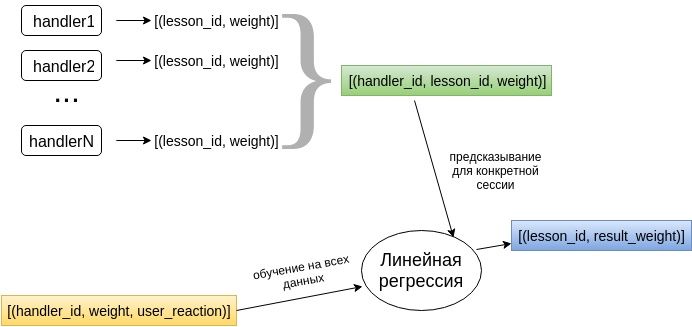
\includegraphics[width=\linewidth]{images/handlers_scheme_short.png}}
    \end{figure}

\end{frame}


\begin{frame}\frametitle{Адаптивные рекомендации: \\MathsGarden}

    \bigskip
    MathsGarden.com
    
    \begin{itemize}
        \item Item Response theory
        \item Elo chess rating \\$\hat{\theta_j} = \theta_j + K(S_j - E(S_j))$
        \item High speed, high stakes
    \end{itemize}
    
    \begin{figure}[t]
      \centering
      \subfloat[начальный экран]{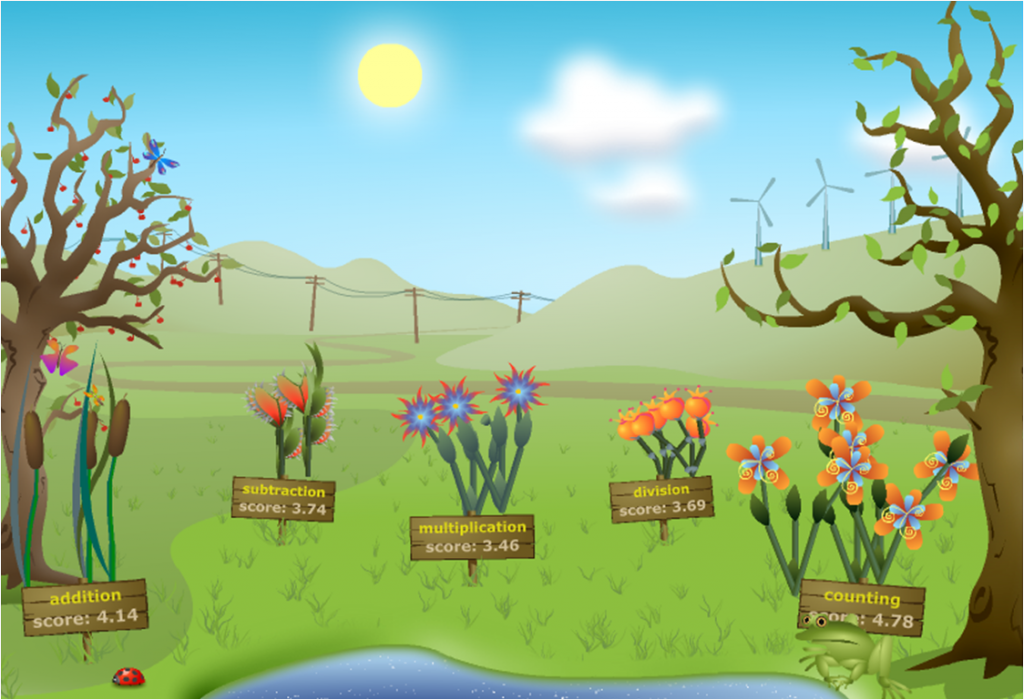
\includegraphics[width=0.4\textwidth]{images/mathsgarden.png} \label{fig_mathsgarden1}}
      \hfill
      \subfloat[решение задачи]{
\includegraphics[width=0.5\textwidth]{images/mathsgarden_quiz.png} \label{fig_mathsgarden2}}
      
    \end{figure}
    
\end{frame}


\begin{frame}\frametitle{Оценка: обычные рекомендации}
\normalsize
    \begin{figure}
    \begin{table}[htp]
        \begin{tabular}{c | r }
          \hline
          Метрика & Значение \\
          \hline		
          \hline
          Число сессий & 381868 \\
          Число сессий с реакцией & 18066 \\
          Процент сессий с реакцией &  4.7\% \\
          Число открытых рекомендаций (из 20) & 1.6 \\
          Пройденная часть урока & 0.52 \\
          Число отказов от рекомендации & 184 \\\hline
        \end{tabular}
    \end{table}
%
      \centering
      \subfloat[открыто ссылок]{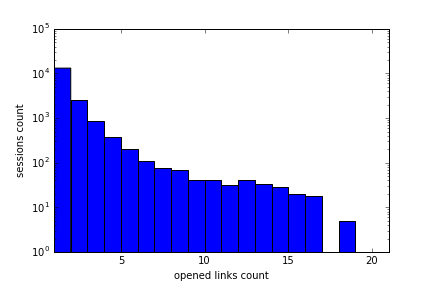
\includegraphics[width=0.5\textwidth]{images/home_page_opened_links_number_hist.png}}
      \hfill
      \subfloat[пройденная часть урока]{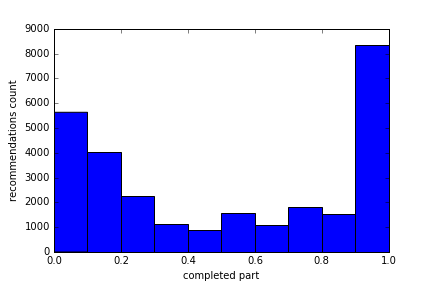
\includegraphics[width=0.5\textwidth]{images/home_page_completed_part_hist.png}}
    \end{figure}
\end{frame}


\begin{frame}\frametitle{Оценка: контекстные рекомендации}
\normalsize
    \begin{figure} 
    \begin{table}
        \centering
        \begin{tabular}{ c | r }
          \hline
          Метрика & Значение \\
          \hline		
          \hline
          Число сессий & 26995 \\
          Число сессий с реакцией & 15125 \\
          Процент сессий с реакцией &  56\% \\
          Число открытых рекомендаций (из 5) & 1.48 \\
          Пройденная часть урока & 0.5 \\
          Число отказов от рекомендации & 0 \\
          \hline  
        \end{tabular}
    \end{table}
%
      \centering
      \subfloat[открыто ссылок]{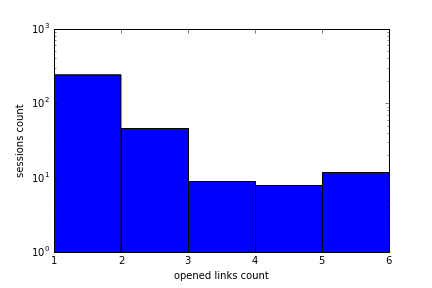
\includegraphics[width=0.5\textwidth]{images/context_opened_links_number_hist.png}}
      \hfill
      \subfloat[пройденная часть урока]{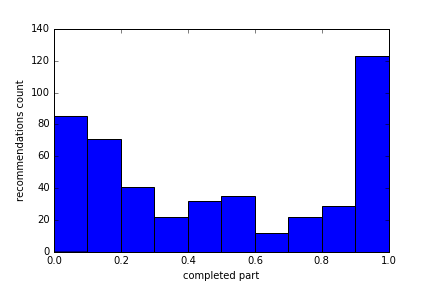
\includegraphics[width=0.5\textwidth]{images/context_completed_part_hist.png}}
    \end{figure}
\end{frame}


\begin{frame}\frametitle{Оценка: адаптивные рекомендации}
\bigskip
\normalsize
    \begin{figure}
    \begin{table}
        \centering
        \begin{tabular}{c | r}
          \hline
          Метрика & Значение \\
          \hline	
          \hline	
          Число сессий & 1511 \\
          Число пользователей & 246 \\
          Реакций "решено" & 1329 \\
          Реакций "слишком просто" & 95 \\ 
          Реакций "слишком сложно" & 87 \\
          MSE предсказания исхода & 0.22 \\
          
         \hline  
        \end{tabular}
    \end{table}
% Также было исследовано, действительно ли ошибка предсказания для конкретного пользователя или задачи уменьшается со временем. Для этого ошибки были усреднены по пользователям (рисунок \ref{fig:adapt1}) и по задачам (рисунок \ref{fig:adapt2}). На получившихся графиках наблюдается явное, хоть и не равномерное, убывание ошибки.
    
      \centering
      \subfloat[пересчет знаний пользователя]{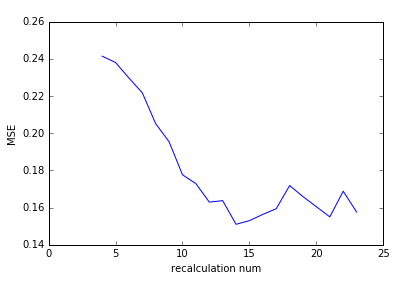
\includegraphics[width=0.45\textwidth]{images/mse_user_skill.png}}
      \hfill
      \subfloat[пересчет сложности задачи]{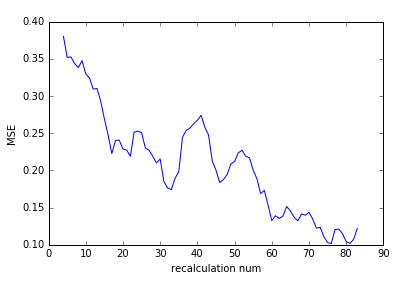
\includegraphics[width=0.45\textwidth]{images/mse_quiz_difficulty.png}}
    \end{figure}
\end{frame}


\begin{frame}\frametitle{Результаты}
\Large
    \begin{itemize}
        \item Рекомендательная система спроектирована, реализована, работает на Stepic.org
        \medskip
        \item Простые, контекстные и \\адаптивные рекомендации
        \medskip
        \item Гибкая система хендлеров
    \end{itemize}

\end{frame}

\end{document}